%!TEX root = ../thesis.tex
%*******************************************************************************
%****************************** Metodologia *********************************
%*******************************************************************************


\chapter{Metodología}
El desarrollo del software requiere de una metodología de trabajo colaborativo basado en una serie de herramientas de contenerización y orquestación de manera eficiente, extensible y reproducible.

\section{Software y plataformas}
A lo largo de este proyecto se han utilizado una serie de softwares y plataformas para el desarrollo de la nueva herramienta, clasificados en diferentes grupos. Dentro de estos conjuntos se encuentran explicados con más detalle los procesos que corresponden según las aplicaciones que se utilizaron.  Estas tareas se llevaban a cabo de forma diaria y se solían efectuar cada cierto tiempo. Estos procesos se dividen en tres: (1) actualización de ficheros, (2) trabajo colaborativo e (3) integración continua.

Antes que nada, se debe de tener en cuenta que los procesos están representados mediante diagramas de secuencia. Por ello, la lectura debe realizar de izquierda a derecha y de arriba a abajo. Las líneas discontinuas corresponden a las notificaciones o mensajes intercambiables que son enviados y recibidos entre distintos actores, y las líneas continuas corresponden a las operaciones que realiza y recibe cualquier actor. Además, con ello podemos relacionar la activación y desactivación del actor cuando éste envía o realiza cualquier operación. Finalmente, entre actores aparecen expresiones como condicionantes o alternativas (alt), opcionales (opt) y bucles o ciclos (loop), es decir, una operación que se repite tantas veces sea necesario o quiera el usuario. Y no menos importante, los actores son los softwares o plataformas utilizados durante el proceso.

\subsection{Control de versiones}
Todas las modificaciones que surgían de uno o varios archivos a lo largo de una tarea, se utilizaba el control de versiones que se encargaba de registrarlas. Gracias a este sistema, se tenía la posibilidad de recuperar una versión antigua en cualquier momento. Para ello se han utilizado dos tipos de sistemas de control:
\begin{itemize}
\item\textbf{Git}: permite tener un control de las versiones que se han distribuido con código abierto y libre, con mayor rapidez y eficacia, sobre el repositorio (lugar en el que se almacenan todos los archivos necesarios de una investigación) en el que estamos trabajando. Por otro lado, este sistema proporciona la posibilidad de replicar y actualizar el repositorio de trabajo, además de añadir, eliminar, mover o reemplazar cualquier archivo. La ventaja de este tipo de sistemas es que se puede crear una rama (branch) colaborativa del repositorio original para tener un aseguramiento de los datos, ya que si en cualquier momento se registra algún problema o éstos se dañan, existe la posibilidad de volver a restaurarlos sin ningún problema desde el repositorio original. Así pues, se creó una nueva rama colaborativa paralela\footnote{\url{https://github.com/andrearosado/pg_landmetrics}} a la rama original del proyecto para operar y modificar sin el riesgo de que los archivos originales fueran dañados. Una vez finalizados y revisados todos los cambios, se procedía a unirlos al repositorio original.
\item\textbf{GitHub}: es una plataforma de desarrollo que alberga proyectos de software, como es el caso del proyecto SIOSE-INNOVA\footnote{\url{https://github.com/siose-innova/pg_landmetrics}}, y almacena de forma pública todo el código, trabajando de forma colaborativa utilizando el sistema de control de versiones de Git. En este caso, su presentación es más visual e interactiva, a través de una interfaz web.
\end{itemize}

Una de las tareas diarias que corresponde a esta subsección es la actualización de ficheros de la extensión. El proceso consistía en que desde la máquina local Git(local) el usuario ejecutaba un comando pull que se encargaba de obtener la última versión del propio repositorio y de revisar si han habido cambios desde la última actualización (este paso es opcional en el caso de que no se tengan los ficheros actualizados pero si se tiene la última versión, no hace falta ejecutar el anterior comando). Cuando la máquina local tenía la última versión, se iniciaba un loop, es decir, el usuario editaba los ficheros de su sistema las veces que eran necesarias. Hechas estas modificaciones, se añadían y actualizaban los ficheros mediante el comando commit, obteniendo a continuación un hash (identificador único) por cada cambio que se había realizado durante el proceso. A partir de aquí, el loop finalizaba si el usuario decidía que no habían más modificaciones que realizar. Finalmente, desde la máquina local, el usuario subía todos los cambios realizados a su propio repositorio y así tener una nueva versión actualizada (ver figura \ref{fig:diary}).


\begin{figure}
\begin{center}
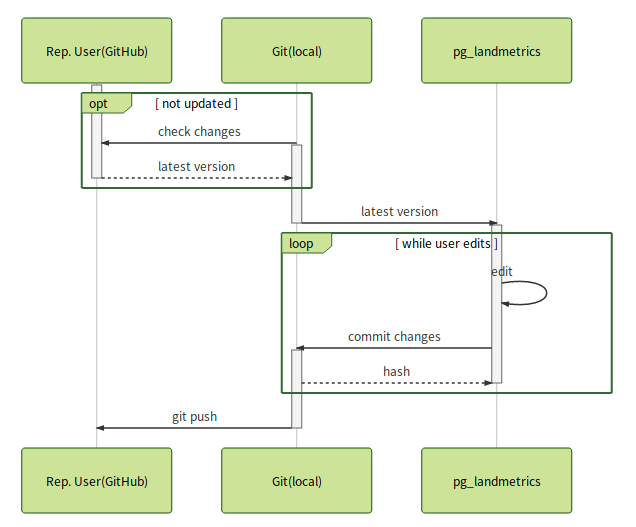
\includegraphics[width=0.9\textwidth]{Metodologia/Figs/diary.png}
\caption{Flujo de proceso de actualización de ficheros. \label{fig:diary}}
\end{center}
\end{figure}

Otro de los procesos, que comparte esta y la siguiente subsección, corresponde al trabajo colaborativo de los usuarios entre sus propios repositorios y el repositorio Upstream (original) del proyecto. Desde el punto de vista más técnico, una de las primeras tareas era realizar un fork, es decir, una copia de todos los ficheros del repositorio Upstream a un nuevo repositorio del propio usuario. La ventaja de esto es que si en cualquier momento el repositorio del usuario sufría algún contratiempo, se podía volver a realizar un fork del repositorio Upstream. A continuación, si no había una copia en la máquina local Git (local), se ejecutaba el comando clone para obtener una copia de la última versión de todos los ficheros del repositorio del usuario. En el caso de que los ficheros no estaban actualizados, se ejecutaba una nueva instrucción donde Git(local) revisaba las últimas modificaciones y, si no los tuviera actualizados, se obtenía su última versión (estos últimos procesos son alternativos, ya que depende del estado de los ficheros). A partir de aquí, el sistema de ficheros quedaba actualizado y se iniciaba el proceso de trabajo colaborativo. En este punto, se producía un loop cada vez que el usuario editaba ficheros, añadía y actualizaba en la máquina local y finalmente, recibía un hash correspondiente a cada modificación que se había realizado. Una vez se hechos todos los cambios, éstos se subían al propio repositorio y en este momento el propio repositorio del usuario estaba por delante del repositorio Upstream ya que éste no tenía los últimos cambios guardado y el loop terminaba ya que no habían más modificaciones que realizar. Ahora es cuando interviene el trabajo colaborativo, es decir, desde el propio repositorio del usuario se enviaba una petición al repositorio Upstream para emparejar ambos a través de la función pull request desde la plataforma de GitHub. Si la petición era aceptada por el personal encargado del repositorio Upstream, el usuario ejecutaba el comando merge (unión) y recibía una notificación de sincronización completada. Finalmente los repositorios quedaban sincronizados y los ficheros con la última versión. Se volvían a subir los cambios al propio repositorio del usuario y se recibía una notificación de que los cambios habían sido correctos. Todo esto queda dentro de un loop hasta que el usuario decidía que no habían más cambios que realizar o ficheros que actualizar (ver figura \ref{fig:pullrequest}).

\begin{figure}
\begin{center}
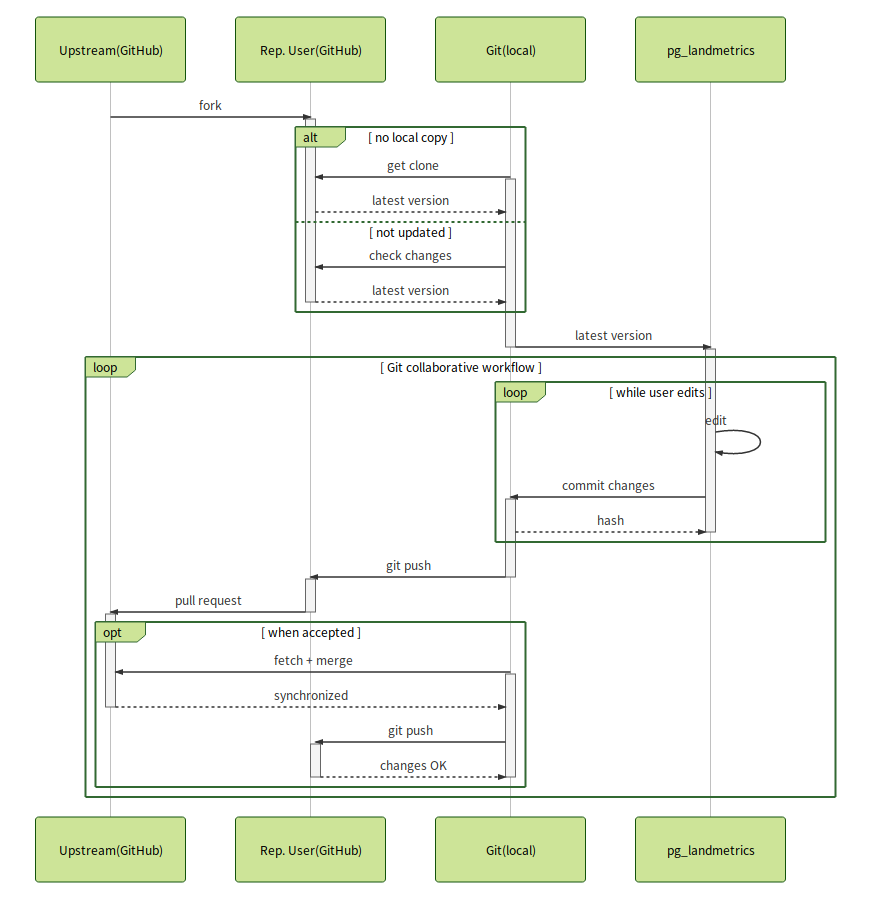
\includegraphics[width=0.9\textwidth]{Metodologia/Figs/pullrequest.png}
\caption{Flujo de proceso de trabajo colaborativo entre repositorios. \label{fig:pullrequest}}
\end{center}
\end{figure}


\subsection{Contenerización y orquestación de servicios}
Uno de los objetivos de la extensión era obtener un alto grado de reproducibilidad y, por ello se ha llevado a cabo la virtualización de un sistema operativo a través de contenedores\footnote{El uso de contenedores es relevante para la reproducibilidad, por eso se evalúan los siguientes criterios objetivos: portabilidad (se pueden reproducir en máquinas cuyos contenedores despliegan recursos compartidos), empaquetado (el software y los datos están compilados en una imagen binaria), reutilización de componentes (distribución entre usuarios de las imágenes sin necesidad de progresos intermedios), distribución (distribución de imágenes a través de plataformas) y versionado (integración de sistema de control de versiones en los archivos para la automatización la compilación de datos) (Boettiger, 2015).} Docker (ver figura \ref{fig:docker}).

\begin{figure}
\begin{center}
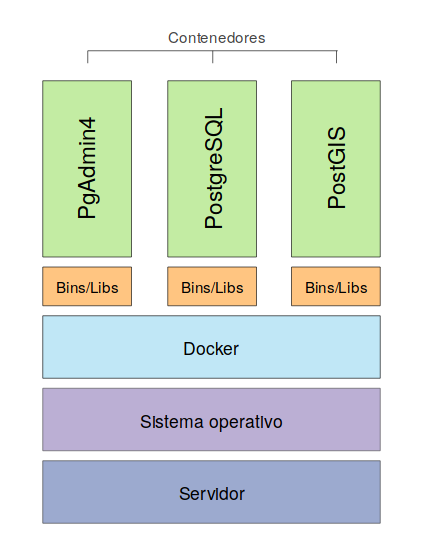
\includegraphics[width=0.5\textwidth]{Metodologia/Figs/docker.png}
\caption{Contenerización del sistema operativo. \label{fig:docker}}
\end{center}
\end{figure}

Se han utilizado los siguientes elementos:
\begin{itemize}
\item\textbf{Docker}: es un servicio de integración continua de código abierto que automatiza el despliegue de ficheros de configuración de aplicación en contenedores facilitando la virtualización en el sistema operativo en cualquier máquina con Docker instalado. Este servicio permitió la portabilidad de las aplicaciones y la reproducibilidad del proyecto en un entorno de trabajo con todos los softwares, configuraciones y datos necesarios, con la ventaja de reproducirlo en cualquier máquina.
\item\textbf{Docker Hub}: es una biblioteca digital donde se almacenan todas las imágenes Docker de aplicaciones en distintos repositorios. Desde aquí se obtuvieron las imágenes de las aplicaciones que se utilizaron.
\item\textbf{Docker-compose}: es un fichero de configuración que despliega todos los servicios que sean necesarios durante el desarrollo de manera rápida y eficaz.
\end{itemize}


Otro de los procesos, que corresponde a esta subsección, es la integración continua del proyecto que conlleva la ejecución de control de versiones y la automatización. Desde el punto de vista del usuario, se ejecutaba el comando  docker-compose build si la extensión había sido modificada. En el caso de que no estuviera modificada y no fuera necesario volver a construir el Docker-compose, solamente era necesario ejecutar el comando docker-compose up para iniciarlo. A partir de aquí, el Docker-compose orquestaba y se ocupaba de lanzar dos contenedores: PostgreSQL/PostGIS y PgAdmin. Una vez han sido lanzados dichos contenedores y se han recibido las notificaciones de que la conexión había sido satisfactoria, se iniciaba un loop mientras el usuario realizaba consultas a los contenedores. A continuación, ambos contenedores realizaban las consultas entre ambos y luego se enviaban al usuario los resultados de las consultas acompañado de una vista previa de ellos. Cuando ya eran adquiridos todos los resultados deseados, el loop se terminaba y se ejecutaba el comando docker-compose down para que el Docker-compose dejase de funcionar y el usuario recibiese una notificación por parte de este actor de que había sido “apagado” sin problema (ver figura \ref{fig:ci}).

\begin{figure}
\begin{center}
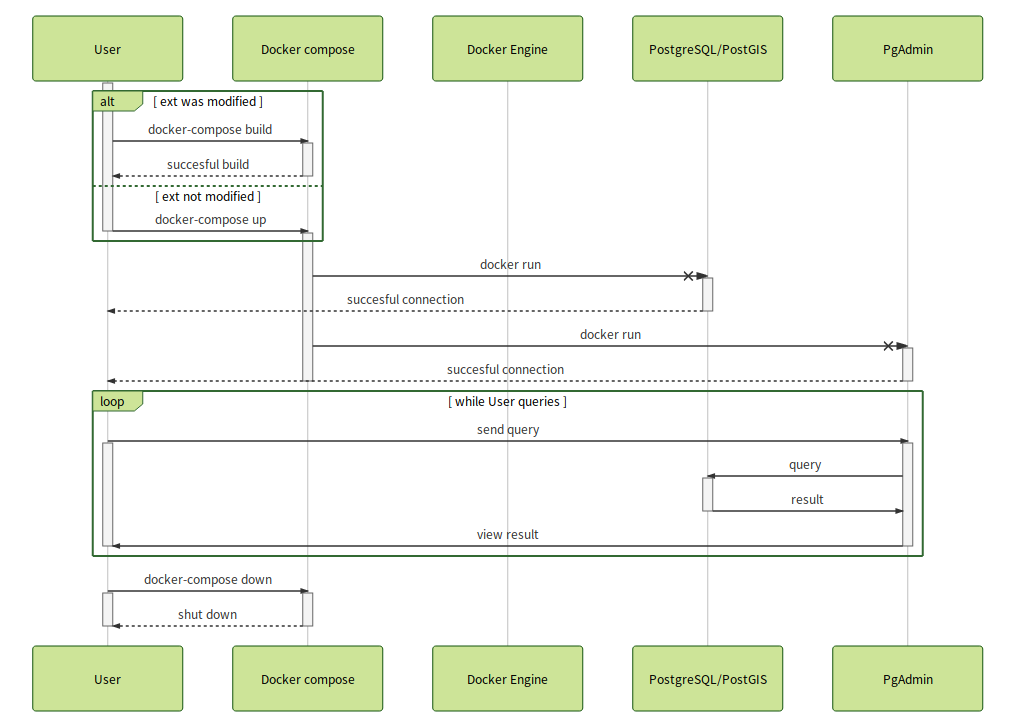
\includegraphics[width=\textwidth]{Metodologia/Figs/ci.png}
\caption{Flujo de proceso de integración continua. \label{fig:ci}}
\end{center}
\end{figure}


\subsection{Extensibilidad}
El \textit{makefile} (fichero encargado de organizar todo el código compilado de todos los programas que se deseen utilizar en la extensión) obtiene la capacidad para ampliar las funcionalidades de cualquier aplicación, como es el caso de la siguiente extensión:
\begin{itemize}
\item\textbf{PostgreSQL/PostGIS}: por un lado, PostgreSQL es un poderoso sistema de bases de datos relacional el cual ayuda a organizar todos los objetos en un conjunto de tablas y, en cuanto a PostGIS es una extensión que añade objetos geográficos a la base de datos relacional de PostgreSQL, pasando a ser una base de datos espacial. Ambas extensiones han permitido la construcción de consultas sobre las bases de datos utilizadas en el proyecto, tanto los de prueba como de los casos de estudio a partir de datos del SIOSE.
\end{itemize}

\subsection{Aplicaciones}
Tanto para el conjunto de datos como para las consultas y funciones de SQL, se utilizaron aplicaciones que realizan unas determinadas tareas:
\begin{itemize}
\item\textbf{PgAdmin4}: es una aplicación de código abierto capaz de administrar y gestionar bases de datos PostgreSQL. En este caso, desde una interfaz web donde se han construido todas las consultas, funciones, agregados,... etc.
\item\textbf{QGIS 2.18}: es una aplicación de escritorio SIG, de código abierto o libre, que analiza, maneja y opera con datos vectoriales, datos ráster y bases de datos. Además facilita la conexión entre las bases de datos espaciales como PostGIS. Gracias a este software se ha elaborado un conjunto de datos que se ha utilizado para comprobar el funcionamiento de las métricas de paisaje.
\end{itemize}

\section{Conjunto de datos}
Antes de seleccionar las métricas de paisaje que han sido utilizadas para complementar el nuevo software, ha sido necesario elaborar y procesar conjuntos de datos que posteriormente se han utilizado para realizar comprobaciones del funcionamiento de las métricas. Así pues, por una parte se ha creado un paisaje ficticio y por otra, se han utilizado los datos del SIOSE de dos zonas de estudio como casos de estudio reales.

Para el paisaje ficticio, se ha digitalizado desde cero todos los polígonos que comprenden esta zona de estudio a partir de herramientas de geoprocesamiento, geometría, vectorial y edición, utilizando QGIS. En la tabla de atributos del shapefile, cada polígono tiene identificador único, geometría, clasificación según el tipo de cobertura del suelo y color según el tipo de categoría al que pertenece.

% Please add the following required packages to your document preamble:
% \usepackage{booktabs}
\begin{table}[]
\centering
\caption{Atributos del primer conjunto de datos.}
\label{my-label}
\begin{tabular}{@{}lll@{}}
\toprule
\textbf{Nombre} & \textbf{Tipo de campo}   & \textbf{Descripción}                    \\ \midrule
gid             & integer                  & Identificador único de cada polígono    \\
geom            & geometry                 & Geometría del polígono                  \\
category        & character varying (text) & Clasificación de la cobertura del suelo \\
svg\_color      & character varying (text) & Color según tipo de categoría           \\ \bottomrule
\end{tabular}
\end{table}

En este paisaje se ha optado por una clasificación de etiquetas simples. En cuanto al color de cada tipo de categoría se ha definido y escogido a partir de los 147 colores que presenta Scalable Vector Graphics (SVG) Specification\footnote{http://www.december.com/html/spec/colorsvg.html}, además del apoyo de la clasificación de colores que especifica la leyenda del Corine Land Cover.v

% Please add the following required packages to your document preamble:
% \usepackage{booktabs}
\begin{table}[]
\centering
\caption{My caption}
\label{my-label}
\begin{tabular}{@{}ll@{}}
\toprule
\textbf{Category}   & \textbf{svg\_color} \\ \midrule
Agricultural area   & lightsalmon            \\
Continuous urban    & lightcoral             \\
Discontinuous urban & lightpink              \\
Forest              & forestgreen            \\
Main road           & gray                   \\
Secondary road      & lightgrey              \\
River               & royalblue              \\
Water body          & mediumblue             \\ \bottomrule
\end{tabular}
\end{table}

Los colores definidos han sido utilizados posteriormente para elaborar y colorear las figuras de la documentación, tanto del trabajo como para la plataforma del proyecto en GitHub, a partir de la función SVG que se ha creado expresamente para ello (véase \label{sec:Documentación de la extensión}).

En el segundo conjunto de datos, se han utilizado los datos del SIOSE de dos zonas de estudio distintas para realizar una comprobación de los resultados de las métricas de paisaje a partir de casos reales y comparar ambos paisajes. La estructura de la tabla de atributos se compone de identificadores únicos, geometría, tipos de coberturas, información en XML, superficie, dos campos para almacenar nueva información y códigos numéricos de producción.

% Please add the following required packages to your document preamble:
% \usepackage{booktabs}
\begin{table}[]
\centering
\caption{Atributos del primer conjunto de datos.}
\label{my-label}
\begin{tabular}{@{}lll@{}}
\toprule
\textbf{Nombre} & \textbf{Tipo de campo}   & \textbf{Descripción}                    \\ \midrule
ID\_POLYGON      & integer                  & Identificador único de cada polígono    \\
GEOMETRY        & geometry                 & Geometría del polígono                  \\
SIOSE\_CODE      & character varying (text) & Tipo de cobertura de cada polígono \\
SIOSE\_XML       & character varying (text) & Información completa del tipo de cobertura \\
& & al que pertenece cada polígono, en formato XML \\


SUPERF\_HA       & character varying (text) & Superficie del polígono en hectáreas \\
OBSER\_C         & character varying (text) & Campo información auxiliar (texto) \\
OBSER\_N         & character varying (text) & Campo información auxiliar (numérico) \\
CODBLQ          & character varying (text) & Código numérico al bloque de producción del SIOSE al que pertenece   \\ \bottomrule
\end{tabular}
\end{table}




% Please add the following required packages to your document preamble:
% \usepackage{booktabs}
% \usepackage{multirow}
\begin{table}[]
\centering
\caption{My caption}
\label{my-label}
\begin{tabular}{@{}lll@{}}
\toprule
\textbf{Nombre}             & \textbf{Tipo de campo}  & \textbf{Descripción}                                               \\ \midrule
ID\_POLYGON                 & string                  & Identificador único de cada polígono                               \\
GEOMETRY                    & geometry                & Geometría del polígono                                             \\
SIOSE\_CODE                 & string                  & Tipo de cobertura de cada polígono                                 \\
\multirow{2}{*}{SIOSE\_XML} & \multirow{2}{*}{string} & Información completa del tipo de cobertura al                      \\
                            &                         & que pertenece cada polígono, en formato XML                        \\
SUPERF\_HA                  & real                    & Superficie del polígono en hectáreas                               \\
OBSER\_C                    & string                  & Información auxiliar (texto)                                       \\
OBSER\_N                    & integer                 & Información auxiliar (numérico)                                    \\
CODBLQ                      & integer                 & Código numérico al bloque de producción del SIOSE al que pertenece \\ \bottomrule
\end{tabular}
\end{table}




\section{Selección de métricas}

\section{Implementación/desarrollo de funciones en PostgreSQL}

\section{Documentación de la extensión}
A lo largo del trabajo, se aplican una serie de lenguajes de marcado para la documentación de la extensión. Pero antes se obtienen conocimientos previos sobre ellos y su funcionamiento para utilizarlos durante el proyecto. Los lenguajes utilizados son:
\begin{itemize}
\item\textbf{Markdown}\footnote{\url{https://github.com/adam-p/markdown-here/wiki/Markdown-Cheatsheet}} es un lenguaje ligero capaz de convertir texto plano a lenguaje HTML. Permite una escritura sencilla y conserva un diseño fácil de lectura. Es compatible con muchas plataformas. Este tipo de lenguaje es utilizado para documentar la extensión en la plataforma de GitHub y la descripción de cada una de las métricas de paisaje.
\item\textbf{TeX}\footnote{\url{https://www.latex-project.org/}} es el lenguaje que se utiliza en el sistema de textos LaTeX y que crea documentos con una alta calidad tipográfica. Se utiliza para escribir artículos o libros científicos, y desde hace tiempo este lenguaje se emplea por un gran número de usuarios. Este tipo de lenguaje es utilizado para redactar este trabajo. Para trabajar con este lenguaje, se utiliza la aplicación Texmaker que se ejecuta desde un contenedor Docker.
\item\textbf{Scalable Vector Graphics (SVG)} es un lenguaje capaz de crear gráficos basados en vectores escalables a partir de archivos vectoriales en 2D y en formato XML. En esta década muchos de los navegadores web utilizan este tipo de lenguaje para sus gráficos. Gracias a este lenguaje, los gráficos no pierden calidad, pueden ser escalables y ocupan menos espacio en la memoria. Este tipo de lenguaje es utilizado para crear las figuras del trabajo.

Por ello, se desarolla una función SQL, como primera propuesta, que dibuja y colorea los gráficos vectoriales que acompañan en el trabajo y en la documentación de la extensión en la plataforma GitHub. Para que las figuras tengan el color correspondiente al tipo de cobertura al que pertenecen, se aplica el código SVG que acompaña a cada polígono en la tabla de atributos del primer conjuntos de datos. La función SVG puede consultarse en el Anexo II.
\item\textbf{Mermaid}\footnote{\url{https://mermaidjs.github.io/}} es un lenguaje de secuencia, que utiliza etiquetas similares a las que son empleadas en el lenguaje de marcado, capaz de generar gráficos a partir de texto por medio de JavaScript. Este tipo de lenguaje se ha utilizado para crear los diagramas de secuencia y el diagrama de Gantt.
\end{itemize}


